\documentclass[a4paper,10pt,titlepage]{article}

\usepackage[utf8]{inputenc}
\usepackage[T1]{fontenc}
\usepackage[danish]{babel}
\usepackage{amssymb}
\usepackage{mathtools}
\usepackage{bchart}
\usepackage{color}
\usepackage{xcolor}
\usepackage{listings}
\usepackage{subcaption}
\usepackage{float}
\usepackage{hyperref}
\hypersetup{%
    pdfborder = {0 0 0}
}

\parindent0em

\lstset{%
frame=single,
numbers=left,
numberstyle=\footnotesize,
tabsize=2,
keepspaces=true,
columns=fullflexible,
basicstyle=\ttfamily\scriptsize,
inputencoding=utf8,
extendedchars=true,
}





\title{Eksamen\\Introduktion til Generisk Programmering}
\author{Henrik Schulz \\ hschu12@student.sdu.dk \\ 011190}
\date{31/1/2017}

\begin{document}
\maketitle
\tableofcontents
\newpage
\section{Forord}
Følgende rapport omhandler implementeringen og test af 
\begin{itemize}
\item
En generisk adjacency-list til at repræsentere grafer
\item
En topologisk sortering af knuder ved brug af en generisk DFS som benytter en Visitor
\end{itemize}
Der er til projektet blevet taget udgangspunkt i kode, som er blevet udleveret af underviseren i DM852 - Introduktion til Generisk Programmering, Jakob Lykke Andersen, i sammenhæng med projektet.
\section{Designvalg}
Der er under implementeringsforløbet blevet foretaget følgende designvalg:
\begin{itemize}
\item
\textbf{Bidirectional:} Udformningen af en bidirectional edge e(u,v) sker ved at lave to directed edge $e(u,v)$ og $e(v,u)$. Dette resulterer i, at når \textit{numEdges(const AdjacencyList \&g)} bliver benyttet, så vil der være 2x antallet af bidirectional edges.
\item
\textbf{edgeOut:} Jeg har valgt at se bort fra den givet struct edgeOut, samt den vector som befinder sig i StoredVertexSimple. I stedet har jeg valgt, at når antallet af kanter ud af en knude skal findes, gøres dette ved at gennemløbe alle kanter i grafen. Hver gang der findes et match tilføjes det til en vector, som i sidste ende vil indeholde de kanter som kræves. Dette gør dog, at når bl.a \textit{outDegree(VertexDescriptor v, const AdjacencyList \&g)} kaldes, så benyttes der $O(E)$ tid i stedet for $O(outDegree)$.
\item
\textbf{AdjacencyList:} Der antages at når \textit{adjacencyList<Directedtag, VertexProp, EdgeProp> (n)} bliver kaldt, oprettes der en adjacencylist som kan indeholde 4 knuder og ikke mere end dette. Dette betyder, at når $addVertex(AdjacencyList\ \&g)$ bliver kaldt, og der allerede er $n$ knuder tilføjet, vil den give en fejl.
\item
\textbf{VertexProp:} Jeg har lavet en bestemt type for vertexProp kaldet Capacity. Dette er en struct som kan indeholde en int, som definerer supply / demand af en knude. Dette er gjort for at have nogle konkrete værdier at arbejde med som label.
\item
\textbf{EdgeProp:} Jeg har lavet en bestemt type for edgeProp kaldet Cost. Dette er en struct som kan indeholde en int, som definerer hvor dyr en given kant er at bruge. Dette er gjort for at have nogle konkrete værdier at arbejde med som label.
\end{itemize}

\section{Problemer/mangler}
\begin{itemize}
\item
\textbf{Segmentation Fault:}Der opstår segmentation fault 11 på visse grafer. Figur 1 viser et tilfælde, hvor DFS visitor fejler efter den har afsluttet alle out-edges til knuden 2.
\begin{figure}[H]
\centering
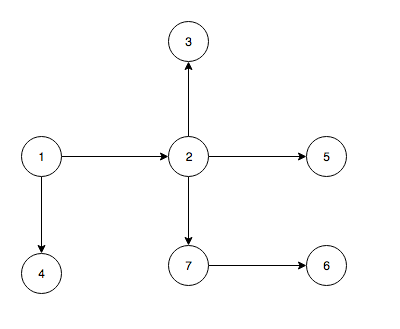
\includegraphics[scale=0.5]{Billeder/SegFaultGraph.png}
\caption{Eksempel på graf der resulterer i segmentation fault}
\end{figure}
Under test3, den topologiske sortering, kan ses at ved mindre ændringer af grafens kanter sker der ingen segmentation fault. Årsagen til fejlen var ikke fundet ved afleveringsdato.
\item
\textbf{Brug af io.hpp:} Dette program er aldrig blevet testet med de metoder der findes i io.hpp.   
\item
\textbf{Ændring af værdi g[e] og g[v]:} Der er ikke blevet implementeret en mulighed for at ændre værdien af hverken VertexProp eller EdgeProp. En værdi kan derfor kun sættes en gang, hvilket er når en knude/kant tilføjes.
\end{itemize}

\section{Implementering}
\subsection{addVertex og addEdge}
Der befinder sig i adjacency\_list.hpp to forskellige addVertex funktioner. Forskellen på de to er hvorvidt en vertexProp skal tilføjes den nyindsatte knude. Ellers tjekker begge funktioner, om der er plads til flere knuder i grafen. Hvis ikke bliver der smidt en fejl og en assert(false) og programmet afbrydes. Ellers får knuden et index som senere bliver dens reference i vores liste af knuder. \\

Ligeledes befinder der sig også fire forskellige addEdge funktioner i adjacency\_list.hpp. Grunden til at der er flere forskellige er fordi der skal være to som håndterer hvorvidt en kant skal have et label eller ej. Derudover skal der også tages højde for hvorvidt en graf er directed eller bidirectional. Dette resultere i to yderligere funktioner. Der bliver benyttet enable\_if til at vurdere hvorvidt funktionen skal være til rådighed eller ej ved compile time. \\
Funktionerne har tilfælles, at de først tjekker for om de knuder, som er involveret, findes. Herefter tjekkes om hvorvidt target og source er samme knude. Sidste tjek er hvorvidt kanten allerede eksisterer. Hvis en af disse tjek fejler, bliver der smidt fejlbesked og lavet et assert(false) som aborter programmet. Hvis alle tjek er gode bliver kanten(e) oprettet og indsat i eList.

\subsection{graph::IncidenceGraph}
\subsubsection{OutEdgeRange}
OutEdgeRange er blevet implementeret med udgangspunkt i \textit{adjacency\ matrix.hpp} egen OutEdgeRange. Begin() og end() er dog blevet ændret, så de nu begge først løber over alle kanter i grafen og samler de kanter som går ud fra den givet vertexDescriptor v. Disse kanter bliver placeret i en vector, som bliver benyttet til at returnere en EdgeRange iterator, som tager udgangspunkt i denne vector egne begin()/end() funktioner.
\subsubsection{source/target}
Source/target funktionerne er ligeledes blevet implementeret med udgangspunkt i \textit{adjacency\ matrix.hpp} matchende funktioner. Source/target tager en edgeDescriptor og returnerer henholdsvis den src eller tar som findes i descriptoren.
\subsubsection{outEdges/outDegree}
Der er i outEdge og outDegree ligeledes blevet taget udgangspunkt i \textit{adjacency\ matrix.hpp}. outEdges returnerer en OutEdgeRange. Når outDegree kaldes, kalder den outEdge, og får derved en OutEdgeRange. Herefter benyttes std::distance til at finde ud af hvor stor denne range er. Dette svarer til outDegree af knuden v.

\subsection{graph::BidirectionalGraph}
\subsubsection{InEdgeRange}
InEdgeRange er blevet implementeret på samme måde som OutEdgeRange. Ligeledes bliver der i både begin() og end() lavet et gennemløb af alle kanter, hvor de kanter som matcher tar=v bliver placeret i en vector. Denne vector bliver derefter brugt til at returnere en iterator.
\subsubsection{inEdges/inDegree}
inEdges og inDegree hænger ligeledes sammen som outEdge og outDegree hænger sammen, og der er derfor taget udgangspunkt i selvsamme funktioner. inEdge returnerer en inEdgeRange. inDegree kan derved på samme måde som outDegree benytte denne range af knuder som returneres til at udregne antallet af inEdges. Dette svarer til inDegree af knuden v.
\subsubsection{degree}
Funktionen degree kalder inDegree og outDegree og ligger deres antal sammen for at skabe den samlede degree af knuden v. Dette returneres.

\subsection{Edge and Vertex Properties}
Jeg har til dette projekt lavet to properties som kan benyttes hvis man ønsker at tilføje enten en cost til en kant, eller en capacity til en knude. Dette er gjort for at have noget konkret at arbejde med i stedet for det mere løse vertexProp og edgeProp.
\subsubsection{EdgeProp: Cost}
Edge property'en Cost indeholder en int som definerer hvor dyr en kant vil være at bruge. Dette kan tilføjes til en kant ved at addEdge bliver kaldt med et ekstra parameter, ep. Dette gør, at der bliver tilføjet et label til kanten som senere kan tilgås ved g[e].
\subsubsection{VertexProp: Capacity}
Vertex property'en Capacity indeholder en int som definerer hvor meget en knude kan "producere". Dette kan tilføjes til en knude ved at kalde addVertex med et ekstra parameter, vp. Dette gør, at der bliver tilføjet et label til knuden som senere kan tilgås ved g[v].

\subsubsection{[ ] operator}
Der befinder sig i adjacency\_list.hpp fire forskellige [ ] operator overloader. To af dem er til at returnere labelet på en kant og de sidste to bruges til at returnere labelet på en knude. Grunden til at der er to af hver, er fordi at der er forskel på om der er en vertexProp/edgeProp at henvise til. Skulle det ske at man kalder g[e] eller g[v] på en graf som er sat til NoProp, så vil den automatisk returnere en int = 0. Dette gøres da programmet ellers ville fejle hvis der forsøges at tilgå variablen vp/ep uden at den er blevet instansieret. Der er blevet benyttet funktionen enable\_if for at vurdere hvilke de fire funktioner der skal være til rådighed. 

\subsection{Toplogisk sortering / Visitor / DFS}

For at implementere DFS metoden er der taget udgangspunkt i den pseudokode som er givet i opgavebeskrivelsen til projektets task2 samt koden der er blevet udleveret til projektet. 
TopoSort() funktionen opretter en ny visitor af typen TopoVisitor for derefter at kalde DFS med den. Da TopoVisitor inheriter fra DfsNullVisitor har jeg valgt at override funktionen \textit{finishVertex(const V\& v, const G\& g)}. Dette gør, at når funktionen bliver kaldt i dfsVisit, bliver denne funktion kaldt i stedet. Funktionen har kun til opgave at indsætte den afsluttede knude i vores outputiterator.\\

\section{Test}
Følgende sektion omhandler de test der er blevet udført. Testene kan findes i mappen graph, og compiles ved hjælp af makefilen.
\subsection{Directed/Bidirectional funktioner}
Til test af en directed og bidirectional graph har jeg benyttet samme graf. Grafen består af 4 knuder og 5 kanter.

Testen til directed graf uden labels (TestDirectedNoProp.cpp), testen til directed graf med labels (TestDirectedProps.cpp), testen til bidirectional graf uden labels (TestBidirectionalNoProp.cpp) og testen til bidirectional grafer med labels (TestBidirectionalProps.cpp) indsætter knuder og kanter så det stemmer overens henholdsvis med figur 2, 3, 4 og 5. Herefter printes der information om grafen: Antal knuder, antal kanter, outDegree for alle knuder, inDegree for alle knuder, degree for alle knuder, source og target på en enkelt kant, getIndex funktionen testes samt [ ] operatoren bliver testet på alle knuder og kanter. Når grafen benytter NoProp til vertexProp og edgeProp vil [ ] operatoren defaulte til at returnere 0, da der ingen værdier er.\\
Alle værdier er blevet tjekket igennem i hånden og stemmer overens de tegnede grafer.

\begin{figure}[H]
\centering
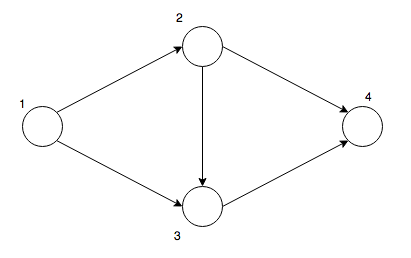
\includegraphics[scale=0.5]{Billeder/GraphDirectedNoProp.png}
\caption{Grafen som bruges til testen af directed graf uden labels.}
\end{figure}
\begin{figure}[H]
\centering
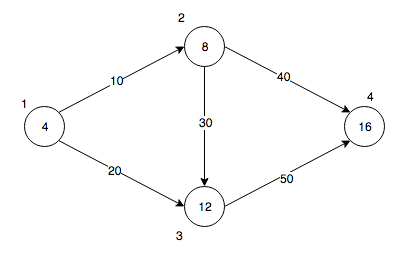
\includegraphics[scale=0.5]{Billeder/GraphDirectedProps.png}
\caption{Grafen som bruges til testen af directed graf med labels.}
\end{figure}

\begin{figure}[H]
\centering
\begin{subfigure}{.5\textwidth}
  \centering
  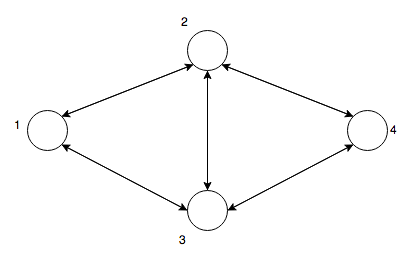
\includegraphics[width=1\linewidth]{Billeder/GraphBidirectionalNoPropSimple.png}
  \caption{}
\end{subfigure}%
\begin{subfigure}{.5\textwidth}
  \centering
  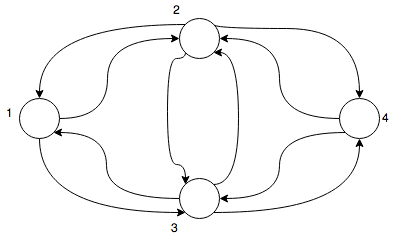
\includegraphics[width=1\linewidth]{Billeder/GraphBidirectionalNoProp.png}
  \caption{}
\end{subfigure}
\caption{a) Viser hvordan grafen normalt vil skulle repræsenteres. b) Viser hvordan grafen bliver repræsenteret i implementeringen.}
\end{figure}

\begin{figure}[H]
\centering
\begin{subfigure}{.5\textwidth}
  \centering
  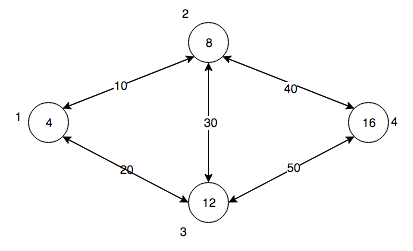
\includegraphics[width=1\linewidth]{Billeder/GraphBidirectionalPropSimple.png}
  \caption{}
\end{subfigure}%
\begin{subfigure}{.5\textwidth}
  \centering
  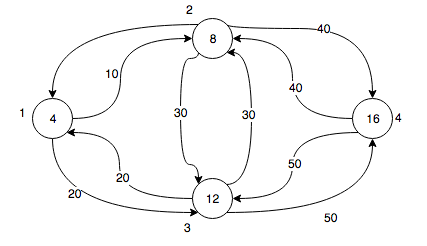
\includegraphics[width=1\linewidth]{Billeder/GraphBidirectionalProps.png}
  \caption{}
\end{subfigure}
\caption{a) Viser hvordan grafen normalt vil skulle repræsenteres. b) Viser hvordan grafen bliver repræsenteret i implementeringen.}
\end{figure}




\subsection{Topologisk Sortering}
For at teste den topologiske sortering blev der lavet to grafer for at teste hvorvidt den fungerede efter hensigten. Begge grafer er blevet løbet igennem i hånden for derefter at være blevet kørt i programmet. De to resultater skulle derefter tjekkes om hvorvidt de stemte overens. Den første graf (figur 1) resulterede dog i en segmentation fault. Den anden graf (figur 6) fungerede dog efter hensigten og resultatet (6,7,1,4,2,5,3) stemte overens med det forventede.
\begin{figure}[H]
\centering
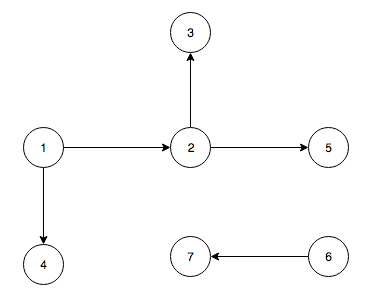
\includegraphics[scale=0.5]{Billeder/DFSGraph.png}
\caption{Grafen som bruges ved test af den topologiske sortering.}
\end{figure}


\subsection{Ikke lovlige operationer}
Denne sektion omhandler de test der er foretaget for at sikre, at visse krav bliver overholdt når der tilføjes kanter og knuder.
\subsubsection{addVertex}
I testen TestAddVertexFAILNoProp.cpp oprettes en AdjacencyList med størrelse 4. Når \textit{addVertex(AdjacencyList \&g)} bliver kaldt for 5. gang resulterer det i en assert failure, da vi forsøger at tilføje en knude som ikke var tiltænkt.\\

I testen TestAddVertexFAILProps.cpp oprettes ligeledes en AdjacencyList med størrelse 4. Når \textit{addVertex(VertexProp vp, AdjacencyList \&g)} bliver kaldt for 5. gang resulterer det i en assert failure, da vi forsøger at tilføje en knude som ikke var tiltænkt.
\subsubsection{addEdge}
I testen TestAddEdgeLargeVertexFAIL.cpp bliver der forsøgt at lave en kant mellem knude 5 og v1 (e(5,v1)). Da AdjacancyList kun er sat op til at skulle have fire knuder, og vi forsøger at lave en kant hvor en af knuderne ikke eksisterer, resulterer det som forventet i et assert(false) kald, som afbryder programmet.\\

I testen TestAddEdgeSameVertexFAIL.cpp bliver der forsøgt at lave en kant mellem v1 og v1 (e(v1,v1)). Da det ikke er muligt at lave en kant der peger på knuden selv (altså source==target) bliver der kaldt et assert(false) som afbryder programmet.\\

I testen TestAddSameEdgeFAIL.cpp bliver der forsøgt at lave en kant som allerede eksisterer (e(v1,v2) og e(v1,v2)). Da dette ikke er lovligt, vil en assert(false) blive kaldt for derefter at afbryde programmet.\\

\section{Forbedringer}
Følgende forbedringer kunne laves:
\begin{itemize}
\item
\textbf{Double Edges ved Bidirectional:} Ved brug af $enable\_if$ funktionen kunne der laves en separat funktion \textit{numEdges(const AdjacencyList \&g)} der deler antallet med to. \\Alternativt: reimplementere hele strukturen så den repræseneterer bidirectional edges anderledes.
\item
\textbf{Properties:} Tilføje flere properties typiske for grafer, samt implementere deres [ ]overloads.
\item
\textbf{Segmentation Faults:} Finde et mønster mellem de grafer, der resulterer i segmentation faults, og finde en løsning på problemet
\end{itemize}

\end{document}